\section{Data Pre-processing}

\subsection{Data Splitting using Sliding Windows}

For time series forecasting, model's performance can differ significantly over different time periods. To ensure the robustness and predictive reliability of my models across different time intervals, this project designs a sliding window approach for data splitting. Rather than segmenting the dataset directly, the sliding window method ensures effective use of overlapping intervals, which is particularly useful for short time series data.

The dataset is divided into training, validation, and test sets within each sliding window. The training set fits predictive models, the validation set is for hyperparameter tuning, and the test set provides an unbiased evaluation of the model's performance.

Figure~\ref{fig:sliding_windows} illustrates the sliding window approach, which shows how overlapping data intervals effectively split the dataset and maximize data usage.

\begin{figure}[h]
\centering
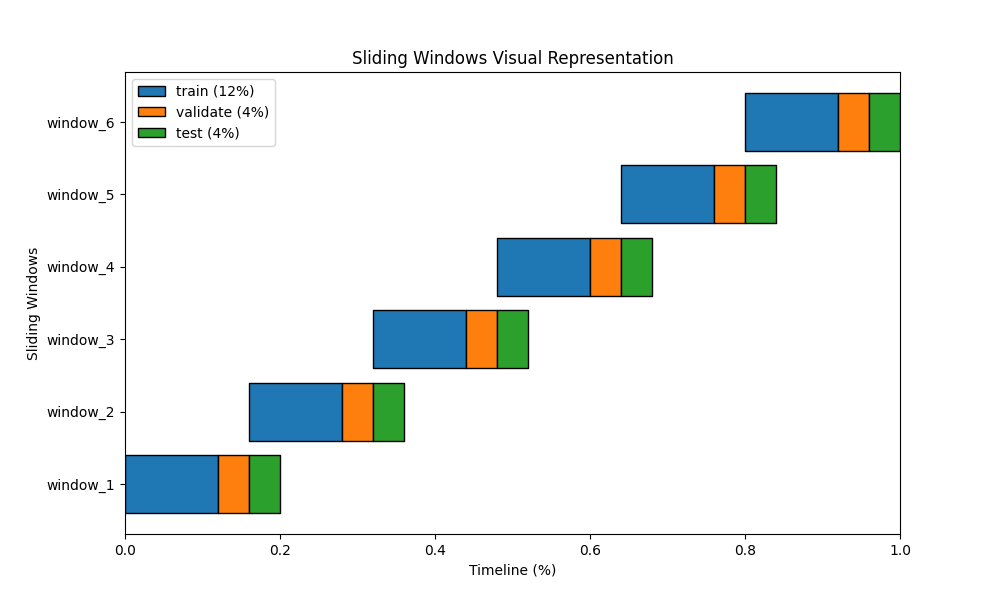
\includegraphics[width=0.8\textwidth]{figures/sliding_windows}
\caption{Sliding Window Data Splitting Strategy}
\label{fig:sliding_windows}
\end{figure}

\subsection{Data Scaling and Normalization}

Data scaling and normalization are important preprocessing techniques aimed at improving model performance, convergence speed, and stability.

\subsubsection{Z-Scale Normalization:}
Z-scale normalization is defined as:
\begin{equation}
z = \frac{x - \mu}{\sigma}
\label{eq:z_scale}
\end{equation}
where \(x\) is a data point, \(\mu\) is the mean, and \(\sigma\) is the standard deviation of the dataset. %This method is suitable when data is normally distributed.

\subsubsection{Min-Max Scaling:}
Min-max scaling rescales data to the range \([0,1]\):
\begin{equation}
x' = \frac{x - \min(x)}{\max(x) - \min(x)}
\label{eq:min_max}
\end{equation}
Min-max scaling is particularly useful when data distribution is not normal.

Note that it is vital to invert the scaling transformation so that the regression metrics are calculated on the original scale.


\subsection{Detrending and Addressing Non-Stationarity}

Time series data often exhibits trends that can negatively affect predictive modeling. Differencing is an effective technique to remove trends and improve the stationarity of time series data. Differencing involves computing the difference between consecutive observations:
\begin{equation}
x'_t = x_t - x_{t-1}
\label{eq:differencing}
\end{equation}
where \(x'_t\) is the differenced data at time \(t\).

However, I failed to invert the differencing transformation for regression metrics calculation, thus the differencing was not applied to regression models.
\textcolor{red}{QUESTION: 提及个人的错误是否合适?}

\subsection{Sequence Transformation}

Long Short-Term Memory (LSTM) models require data structured into sequences. This involves reshaping data into a three-dimensional array:
\begin{equation}
(\text{samples}, \text{timesteps}, \text{features})
\label{eq:reshaping}
\end{equation}
where samples represent the number of independent sequences in the dataset, timesteps represent the number of time intervals within each sample, and features represent the number of variables observed at each time step.

